
%%%%%%%%%%%%%%%%%%%%%%%%%%%%%%%%%%%%%%%%%%%%%%%%%%%%%%
% A Beamer template for HKUST (GZ)                   %
% Based on THU beamer theme                          %
% Author: Yuxuan HU                                  %
% Date: Aug 2024                                    %
% LPPL Licensed.                                     %
%%%%%%%%%%%%%%%%%%%%%%%%%%%%%%%%%%%%%%%%%%%%%%%%%%%%%%

\documentclass[serif, aspectratio=169]{beamer}
%\documentclass[serif]{beamer}  % for 4:3 ratio
\usepackage[T1]{fontenc}
\usepackage[spanish]{babel}
\usepackage{fourier} % see "http://faq.ktug.org/wiki/uploads/MathFonts.pdf" for other options
\usepackage{hyperref}
\usepackage{latexsym,amsmath,xcolor,multicol,booktabs,calligra}
\usepackage{graphicx,pstricks,listings,stackengine}
\usepackage{lipsum}

\author{}
\title{Dinámica Molecular Dirigida por Eventos}
\subtitle{Trabajo Práctico Nro. 3}
\institute{
    Grupo 7: \\
    - Baez, Mauro Leandro (61747)\\
    - Ippolito, Martin Augusto (62510)\\
    - Preiti Tasat, Axel Facundo (62618)\\
}
\date{\small \today}
\usepackage{HKUSTstyle}
\usepackage{blkarray}
\usepackage{caption}
\usepackage{algorithmicx}

% defs
\def\cmd#1{\texttt{\color{red}\footnotesize $\backslash$#1}}
\def\env#1{\texttt{\color{blue}\footnotesize #1}}
% set colors
\definecolor{hkustyellow}{RGB}{167, 131, 55}
\definecolor{hkustblue}{RGB}{0, 56, 116}
\definecolor{hkustred}{RGB}{209, 51, 59}


\lstset{
    basicstyle=\ttfamily\small,
    keywordstyle=\bfseries\color{deepblue},
    emphstyle=\ttfamily\color{deepred},    % Custom highlighting style
    stringstyle=\color{deepgreen},
    numbers=left,
    numberstyle=\small\color{halfgray},
    rulesepcolor=\color{red!20!green!20!blue!20},
    frame=shadowbox,
}

%- --- --- --- --- --- --- --- --- --- --- --- --- --- --- ---
\begin{document}

    \begin{frame}
        \titlepage
        \vspace*{-0.6cm}
        \begin{figure}[htpb]
            \begin{center}
                
\includegraphics[keepaspectratio, scale=0.15]{pic/itba}
            \end{center}\label{fig:figure-itba}
        \end{figure}
    \end{frame}

    \begin{frame}
        \tableofcontents[sectionstyle=show,
            subsectionstyle=show/shaded/hide,
            subsubsectionstyle=show/shaded/hide]
    \end{frame}

% Content --- --- --- --- --- --- --- --- --- --- --- ---
    \section{Ejericico 2}\label{sec:ejer2}


\section{Introducción}\label{sec:introduccion}
\begin{frame}{Simulación regida por tiempo}
    \textbf{Características:}
    \begin{itemize}
        \item 100 partículas posicionadas horizontalmente una al lado de la otra con resortes entre ellas.
        \item Todas las partículas cuentan con la misma masa.
        \item Solo una partícula, la número 100, se mueve sin considerar la fuerza ejercida por las otras.
        \item Las partículas tienen un movimiento principalmente vertical.
    \end{itemize}
\end{frame}

\begin{frame}{Introducción}
    \begin{block}{Diagrama:}
        \begin{figure}
            \centering
            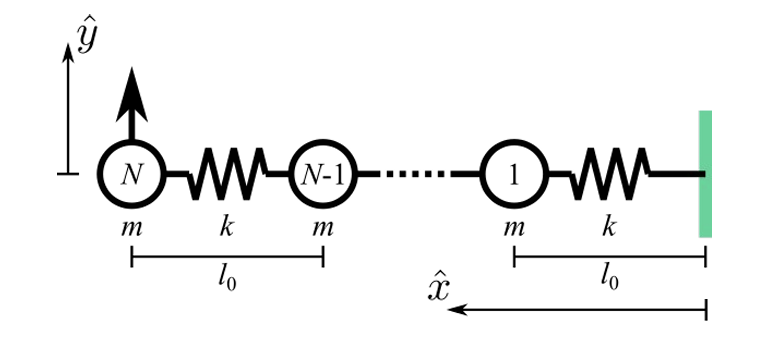
\includegraphics[width=0.8\linewidth]{pic/01-introduccion/diagrama}
            \label{fig:diagrama}
        \end{figure}
    \end{block}
\end{frame}

\begin{frame}{Utilizando Verlet en los pasos temporales}
    \textbf{Fórmulas:}

    \vspace{5pt}
    \begin{equation*}
        r_i(t + \Delta{t}) = 2 r_i(t) - r_i(t-\Delta{t}) + \frac{\Delta{t}}{m_i} f_i(t) + O(\Delta{t}^4)
    \end{equation*}
    
    \vspace{20pt}
    \begin{equation*}
        v_i(t) = \frac{r_i(t+\Delta{t}) + r_i(t-\Delta{t})}{2\Delta{t}} + O(\Delta{t}^3)
    \end{equation*}
\end{frame}

\begin{frame}{Modelo}
    \begin{block}{Fuerzas Partículas 1 a 99}
        \begin{equation*}
            \begin{aligned}
                F_i(t+t_0) &= -k\ (y_i - y_{i-1}) - k\ (y_i - y_{i+1})
            \end{aligned}\label{eq:equation-particles-movement}
        \end{equation*}
        Considerando \( y_0 \) como la constante 0
    \end{block}

    \begin{block}{Partícula 100}
        Siempre seguirá el movimiento: \begin{equation*}A\ sin(\omega t)\end{equation*}
    \end{block}
\end{frame}



%\section{Modelo}
\begin{frame}{Background and Motivation}
    \frametitle<presentation>{Background and Motivation}
    \begin{block}{Why to give a presentation:}
        \begin{itemize}
            \item show the main arguments and results of your work
            \item produce interest to read the full paper/report
            \item goal: be educational and also entertaining
        \end{itemize}
    \end{block}
    \begin{block}{Advantages of using \LaTeX ~with the beamer package:}
        \begin{itemize}
            \item very easy if the report is already written in \LaTeX
            \item different themes which are usable in practice
            \item possibility to create handouts using \emph{beamerarticle}
        \end{itemize}
    \end{block}
\end{frame}

\begin{frame}{Research question}

    this is a Research question.

\end{frame}
    YA SE INCLUYEN EN 01-INTRODUCION
    \section{Implementación}\label{sec:implementacion}
\begin{frame}{Diagrama UML}
\begin{center}
    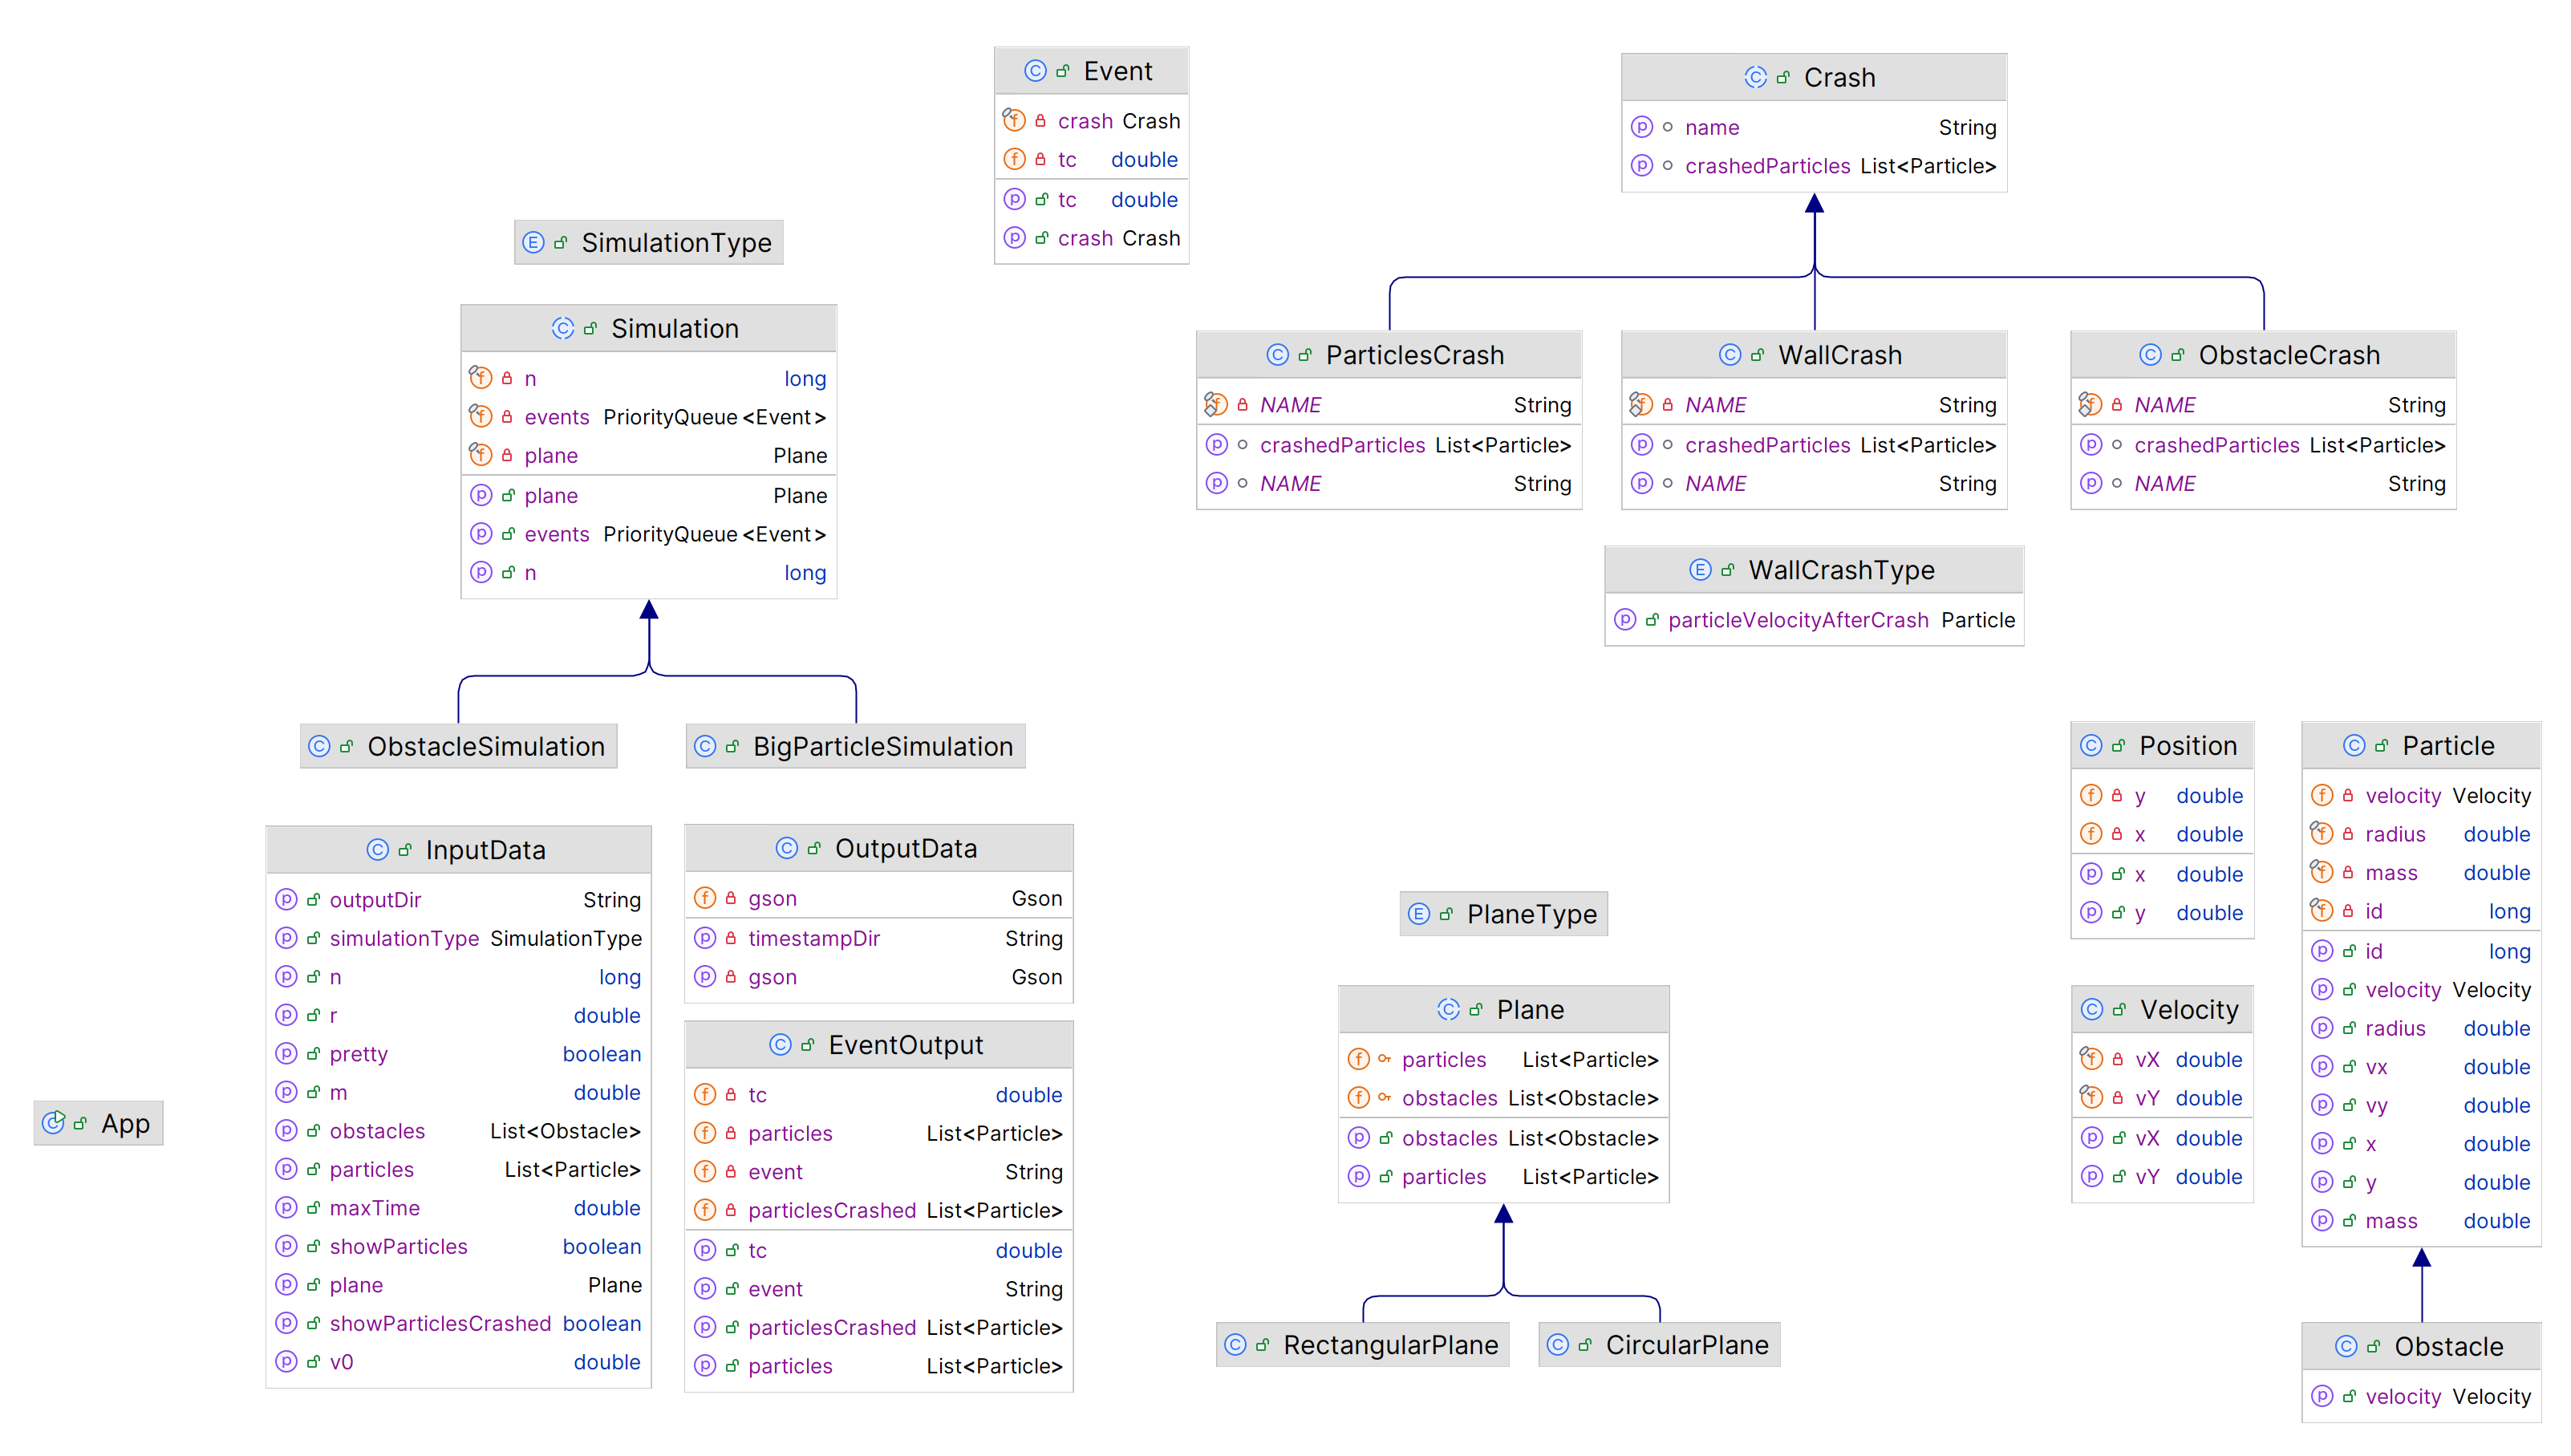
\includegraphics[width=\textwidth]{pic/03-implementacion/UML}
\end{center}
\end{frame}

\begin{frame}{Pseudocódigo}
    \scriptsize{
        \begin{algorithmic}
            \State \text{Generar: campo, defensores y atacante}
            \While{\text{true}}
                \For{\text{cada jugador}}
                    \State \text{Preguntar su dirección objetivo deseada segun heuristica}
                    \State \text{Calcular el vector velocidad en función del modelo operativo y dirección objetivo}
                \EndFor
                \State \text{Pasar dt tiempo}
                \For{\text{cada jugador}}
                    \State \text{Actualizar posición}
                \EndFor
                \If{\text{atacante está sobre límite izquierdo}}
                    \State \text{Emitir evento $try$}
                    \State \text{break}
                \ElsIf{\text{atacante está sobre cualquier otro límite}}
                    \State \text{Emitir evento $out$}
                    \State \text{break}
                \ElsIf{\text{algún defensor se solapa con el atacante}}
                    \State \text{Emitir evento $tackle$}
                    \State \text{break}
                \EndIf
            \EndWhile
        \end{algorithmic}
    }
\end{frame}

    \section{Simulaciones}\label{sec:simulaciones}

\subsection{Parámetros de entrada}\label{subsec:parametros-de-entrada}

Para poder llevar a cabo las simulaciones, se toma en cuenta un conjunto de parámetros de entrada.
Los mismos se pueden categorizar entre fijos y variables, dependiendo de si su valor se mantiene
constante a lo largo de todas las ejecuciones de la simulación para un mismo conjunto de reglas, o no.

Comenzando con los parámetros fijos, se tiene los límites de la matriz ($border$),
en el que se indican los valores máximos y mínimos de las coordenadas de las celdas en dos o tres dimensiones.
Luego, se define la condición de vecindad a partir de dos parámetros:
la forma en la que se consideran las celdas vecinas a una celda en particular, según los modelos mencionados
en~\ref{subsec:definiciones-de-vecindad} ($condition$), y el alcance de la vecindad ($r$).
Con respecto a las reglas de juego, se cuenta con dos parámetros que determinan las posibles cantidades de
vecinos que debe tener una celda para que se mantenga viva ($shouldKeepAlive$),
y para que una celda muerta se convierta en viva ($shouldRevive$); ambos son listas de enteros.
Por último, se determinó el dominio inicial ($initialDomainProportion$), el
cual representa una proporción del área, si es un simulación en dos dimensiones, o del volumen,
si es en tres dimensiones, total de la matriz donde se generan las celdas vivas en el paso temporal 0.
Es decir, siendo $A$ el área o volumen total de la matriz, el dominio inicial es $A \times initialDomainProportion$.

Por otro lado, los parámetros que se varían a lo largo de las simulaciones son la cantidad de pasos temporales
máximos ($maxIter$), y la proporción de densidad de celdas vivas en el dominio inicial ($initialLiveCellsProportion$),
siendo este último un valor entre 0 y 1.


\subsection{Definición de Observables}\label{subsec:observables-posibles}

A continuación, se definen el conjunto de observables, utilizados en la sección \ref{sec:resultados},
para analizar los resultados obtenidos en el equilibrio de las simulaciones realizadas, en función
de la densidad de celdas vivas en el dominio inicial.

\subsubsection{Cantidad de celdas vivas}\label{subsubsec:cantidad-de-celdas-vivas}
Este observable calcula la cantidad de celdas vivas en la matriz en un paso temporal de equilibrio.
Se define como:
\begin{equation}
    \text{Q} = \sum_{i=1}^{x} \sum_{j=1}^{y} \sum_{k=1}^{z} \mathbbm{1}_{\text{viva}}
    \label{eq:cantidad-celdas-vivas}
\end{equation}
donde $Q$ es la cantidad de celdas vivas, $x$, $y$ y $z$ son las dimensiones de la matriz, y $\mathbbm{1}_{\text{viva}}$
es una función indicadora que toma el valor de 1 si la celda en la posición $(i, j, k)$ está viva, y 0 en caso contrario.

\subsubsection{Pendiente de crecimiento de cantidad de celdas vivas}\label{subsubsec:pendiente-de-crecimiento-de-cantidad-de-celdas-vivas}
Este observable calcula la pendiente de cantidad de celdas vivas en la matriz, entre el paso temporal
inicial y el paso temporal de equilibrio.
Se define como:
\begin{equation}
    \text{P}_{\text{Q}} = \frac{Q_{\text{eq}} - Q_{0}}{t_{\text{eq}} - t_{0}}
    \label{eq:pendiente-crecimiento-celdas-vivas}
\end{equation}
donde $P_{Q}$ es la pendiente de crecimiento de cantidad de celdas vivas, $Q_{eq}$ es la
cantidad de celdas vivas en el paso temporal de equilibrio, $Q_{0}$ es la cantidad de celdas
vivas en el paso temporal inicial, $t_{eq}$ es el paso temporal de equilibrio, y $t_{0}$ es el paso temporal inicial.

\subsubsection{Tiempo de convergencia al equilibrio}\label{subsubsec:tiempo-de-convergencia-al-equilibrio}
Este observable calcula la cantidad de pasos temporales que tarda la simulación en converger al equilibrio.
Se define como:
\begin{equation}
    \text{T} = t_{\text{eq}} - t_{0}
    \label{eq:tiempo-convergencia-equilibrio}
\end{equation}
donde $T$ es el tiempo de convergencia al equilibrio, $t_{eq}$ es el paso temporal de equilibrio,
y $t_{0}$ es el paso temporal inicial.

\subsubsection{Distancia de la celda viva más alejada al centro}\label{subsubsec:distancia-de-la-celda-viva-mas-alejada-al-centro}
Este observable calcula la distancia de la celda viva más alejada al centro de la matriz
en el paso temporal de equilibrio.
Se define como:
\begin{equation}
    \text{D} = \max_{i, j, k} \left( \sqrt{(i - x/2)^2 + (j - y/2)^2 + (k - z/2)^2} \right)
    \label{eq:distancia-celda-viva-mas-alejada-al-centro}
\end{equation}
donde $D$ es la distancia de la celda viva más alejada al centro, $x$, $y$ y $z$ son las dimensiones de la matriz,
y $i$, $j$ y $k$ son las coordenadas de la celda en la posición $(i, j, k)$.

\subsubsection{Rapidez de alejamiento de la celda viva más alejada al centro}\label{subsubsec:rapidez-de-alejamiento-de-la-celda-viva-mas-alejada-al-centro}
Este observable calcula la pendiente de la distancia de la celda viva más alejada al centro de la matriz,
entre el paso temporal inicial y el paso temporal de equilibrio.
Se define como:
\begin{equation}
    \text{P}_{\text{D}} = \frac{D_{\text{eq}} - D_{0}}{t_{\text{eq}} - t_{0}}
    \label{eq:rapidez-alejamiento-celda-viva-mas-alejada-al-centro}
\end{equation}
donde $P_{D}$ es la rapidez de alejamiento de la celda viva más alejada al centro, $D_{eq}$ es la
distancia de la celda viva más alejada al centro en el paso temporal de equilibrio, $D_{0}$ es la
distancia de la celda viva más alejada al centro en el paso temporal inicial, $t_{eq}$ es el paso
temporal de equilibrio, y $t_{0}$ es el paso temporal inicial.









    \section{Resultados}\label{sec:resultados}

\begin{frame}
    \begin{center}
        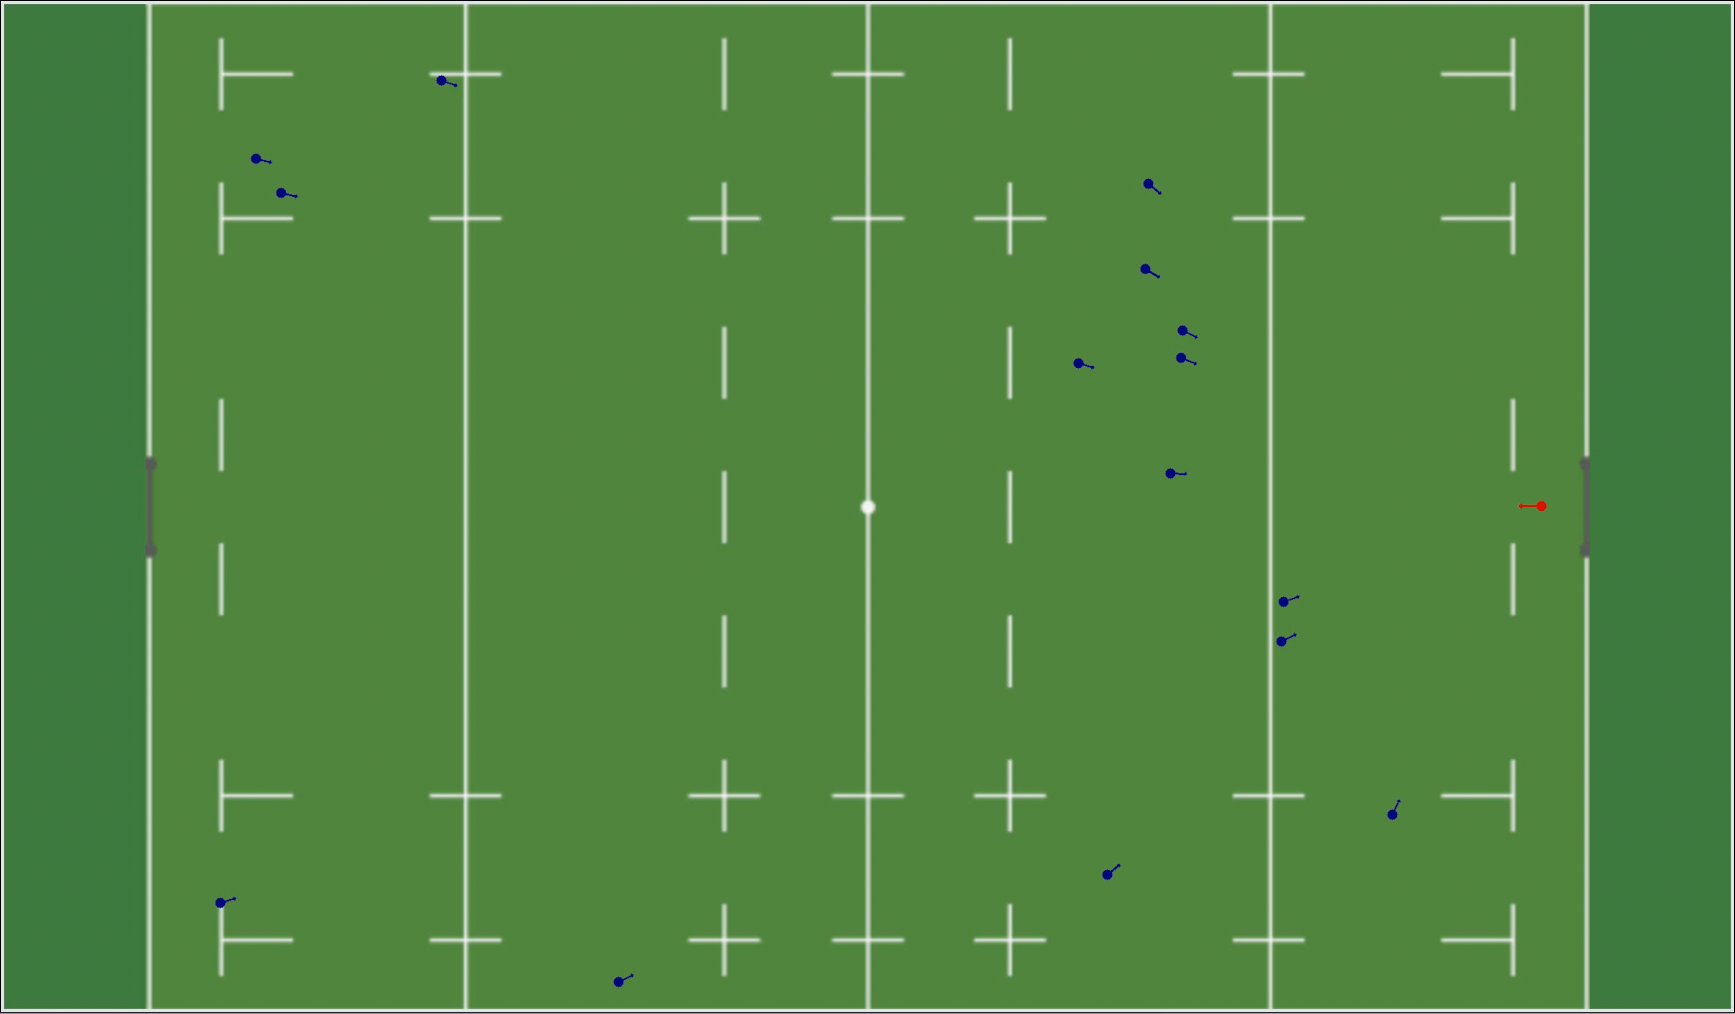
\includegraphics[width=0.9\textwidth]{pic/05-resultados/animation-preview}
    \end{center}
\end{frame}

\begin{frame}{...}
    \begin{center}
        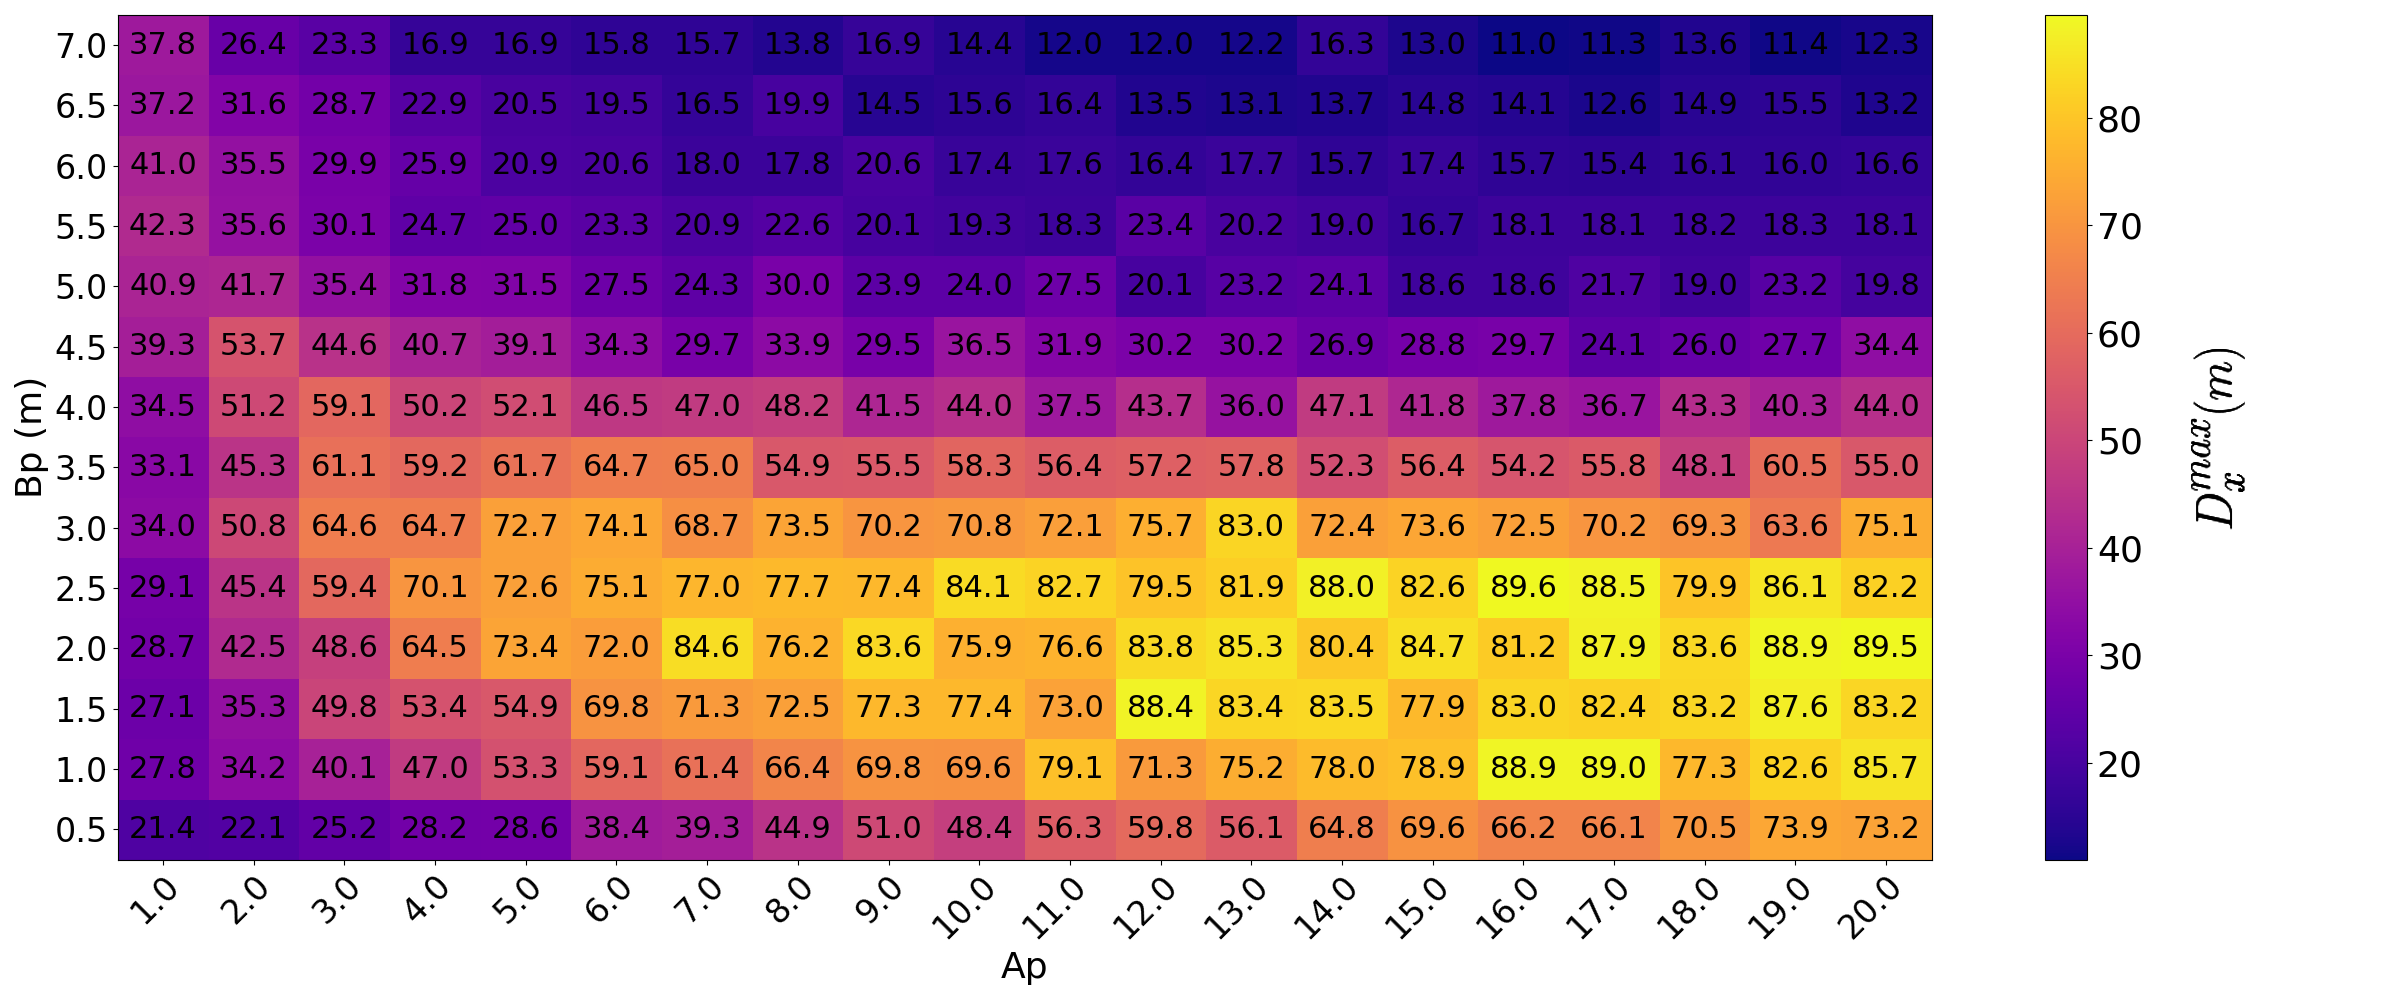
\includegraphics[width=\textwidth]{pic/05-resultados/r1}
    \end{center}
\end{frame}

\begin{frame}{...}
    \begin{center}
        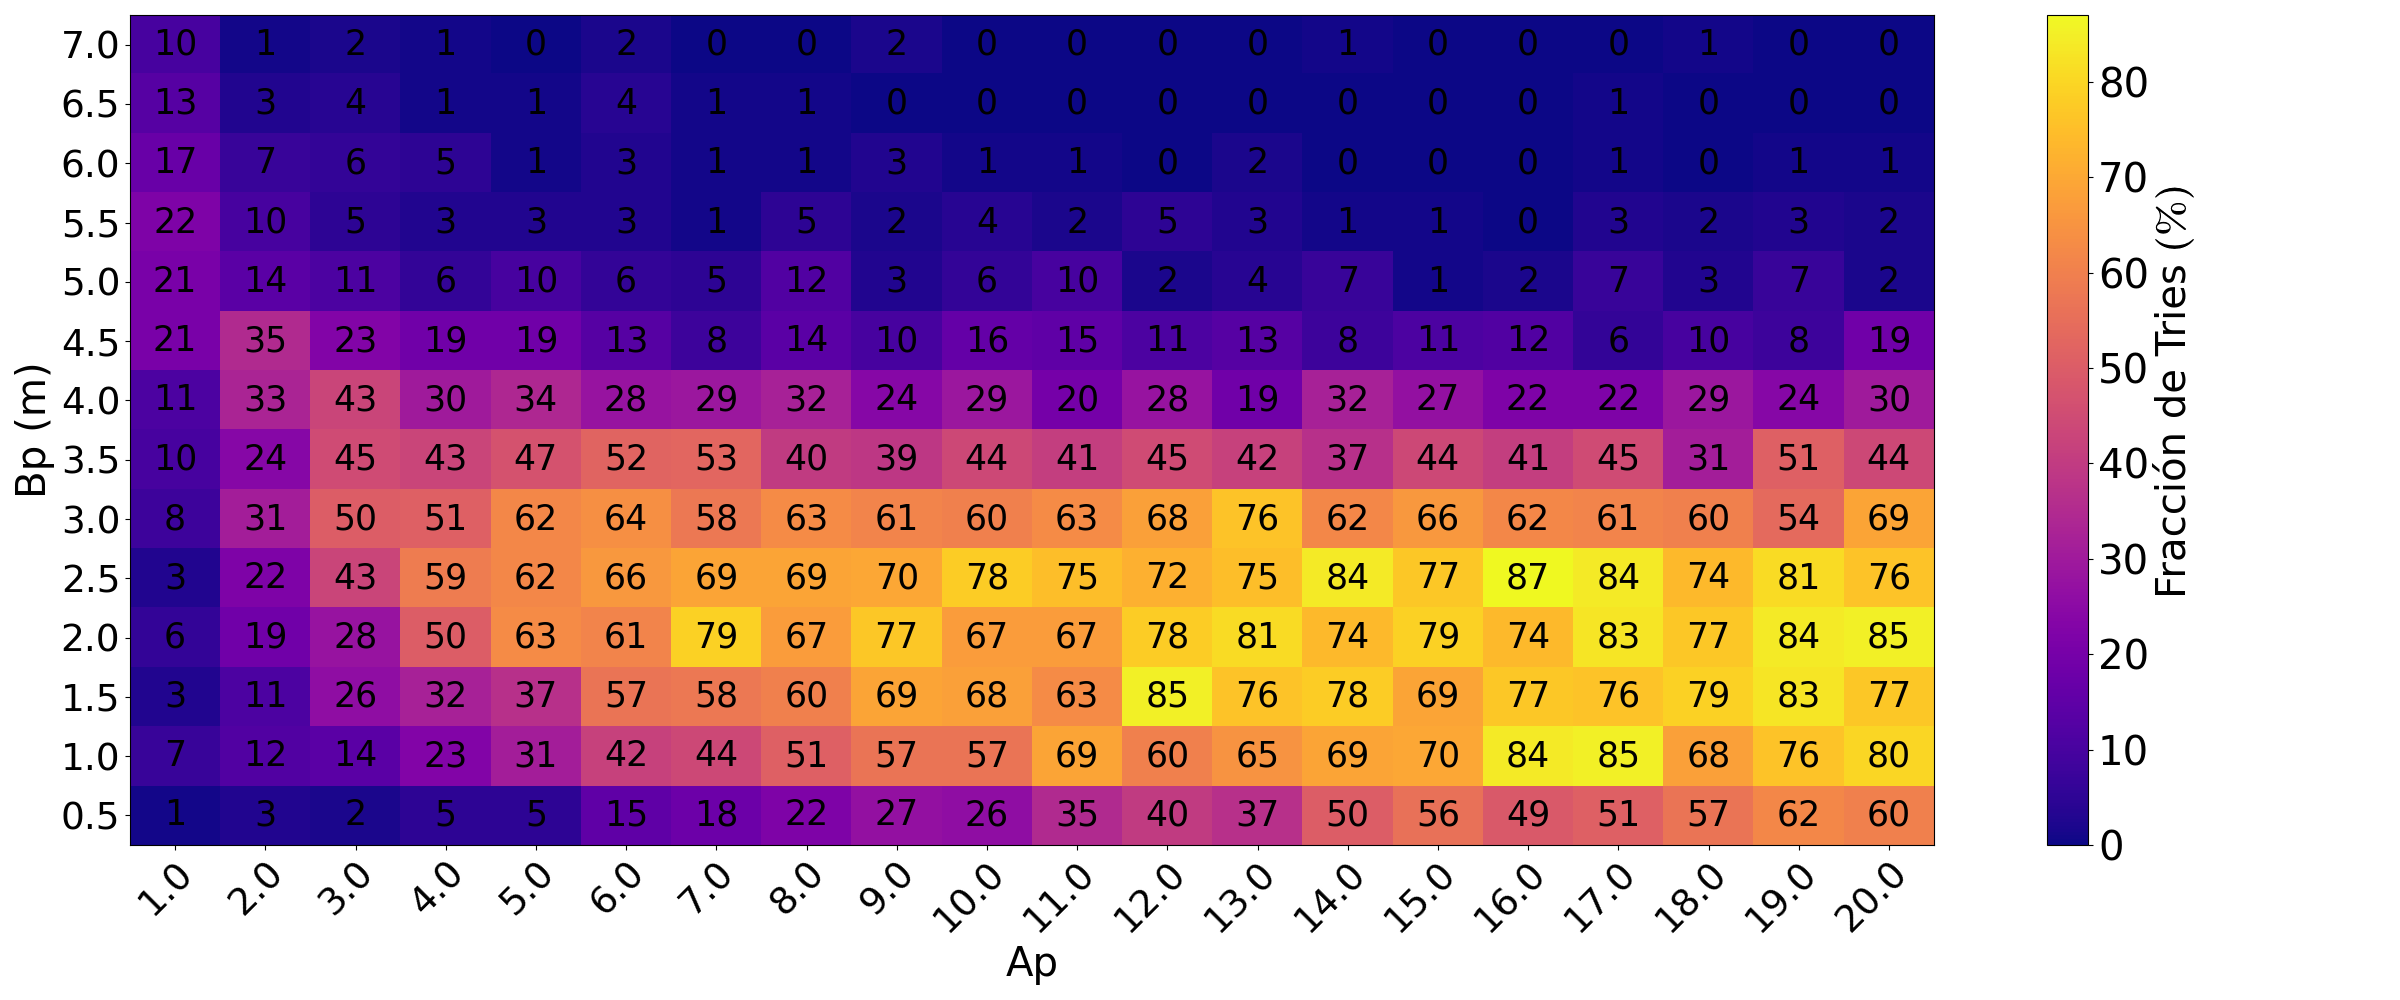
\includegraphics[width=\textwidth]{pic/05-resultados/r2}
    \end{center}
\end{frame}

\begin{frame}{...}
    \begin{center}
        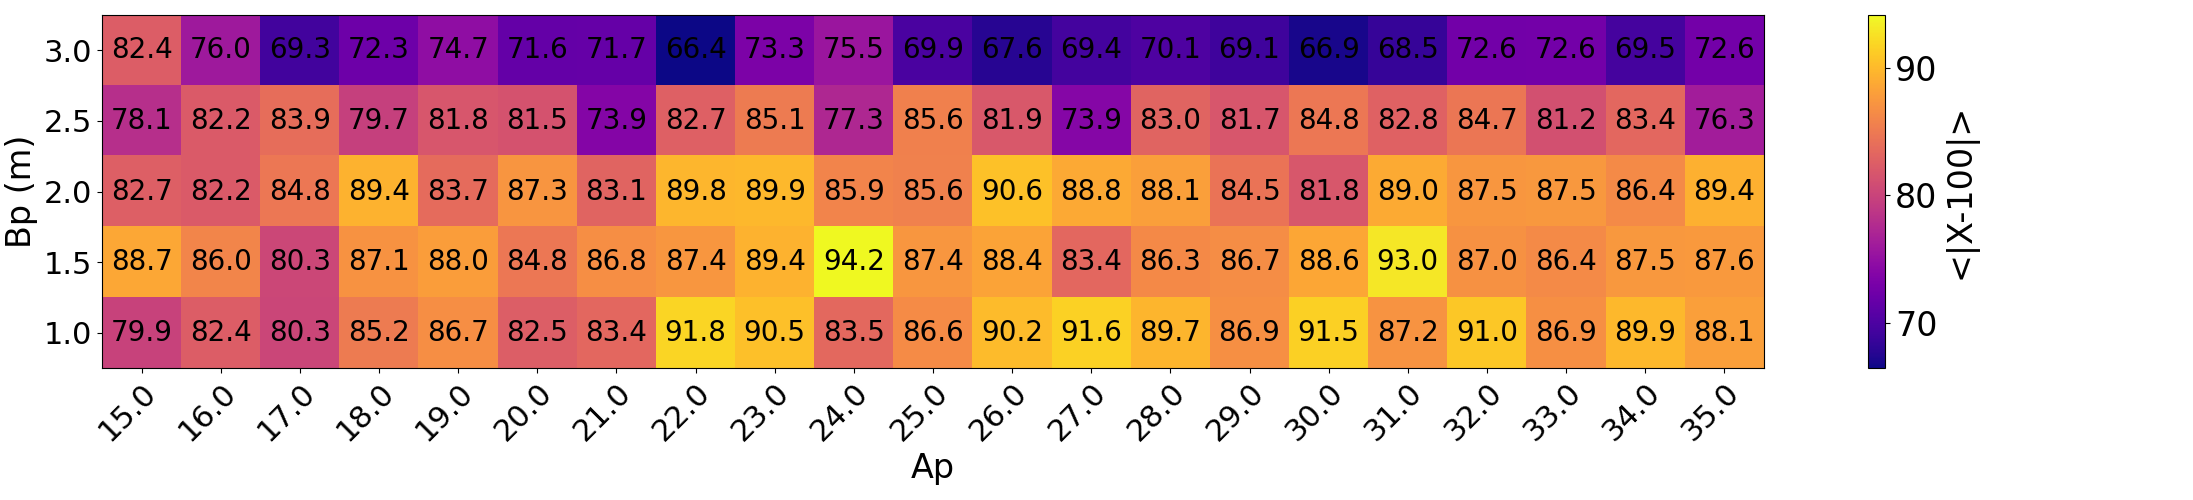
\includegraphics[width=\textwidth]{pic/05-resultados/r3}
        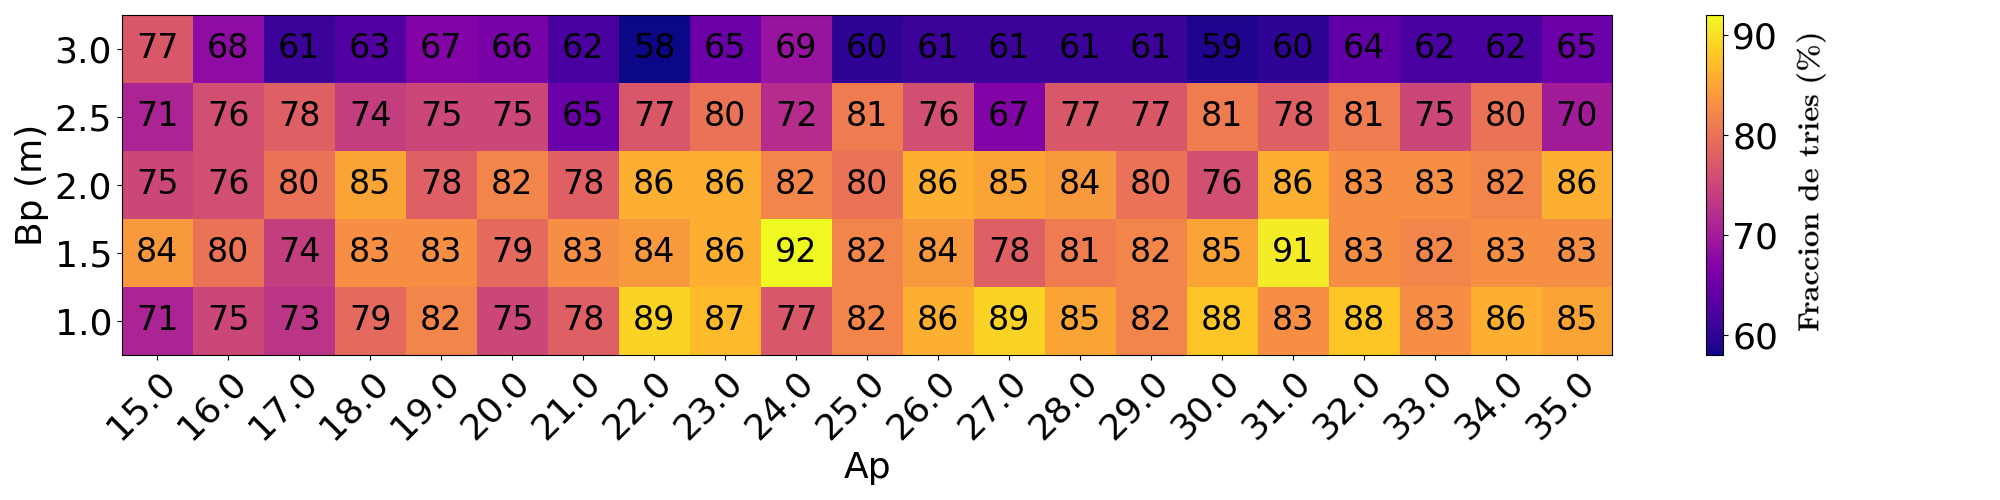
\includegraphics[width=\textwidth]{pic/05-resultados/r4}
    \end{center}
\end{frame}


\begin{frame}{...}
    \begin{center}
        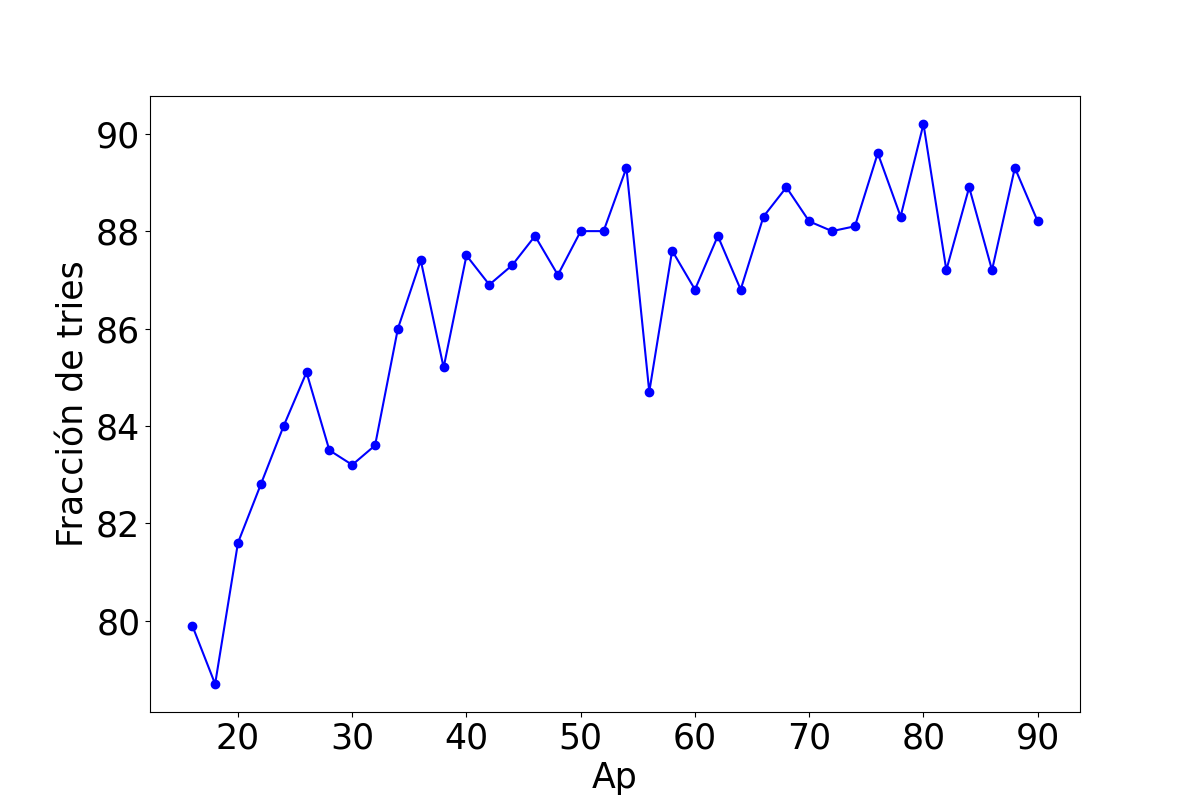
\includegraphics[width=0.75\textwidth]{pic/05-resultados/r5}
    \end{center}
\end{frame}

\begin{frame}{...}
    \begin{center}
        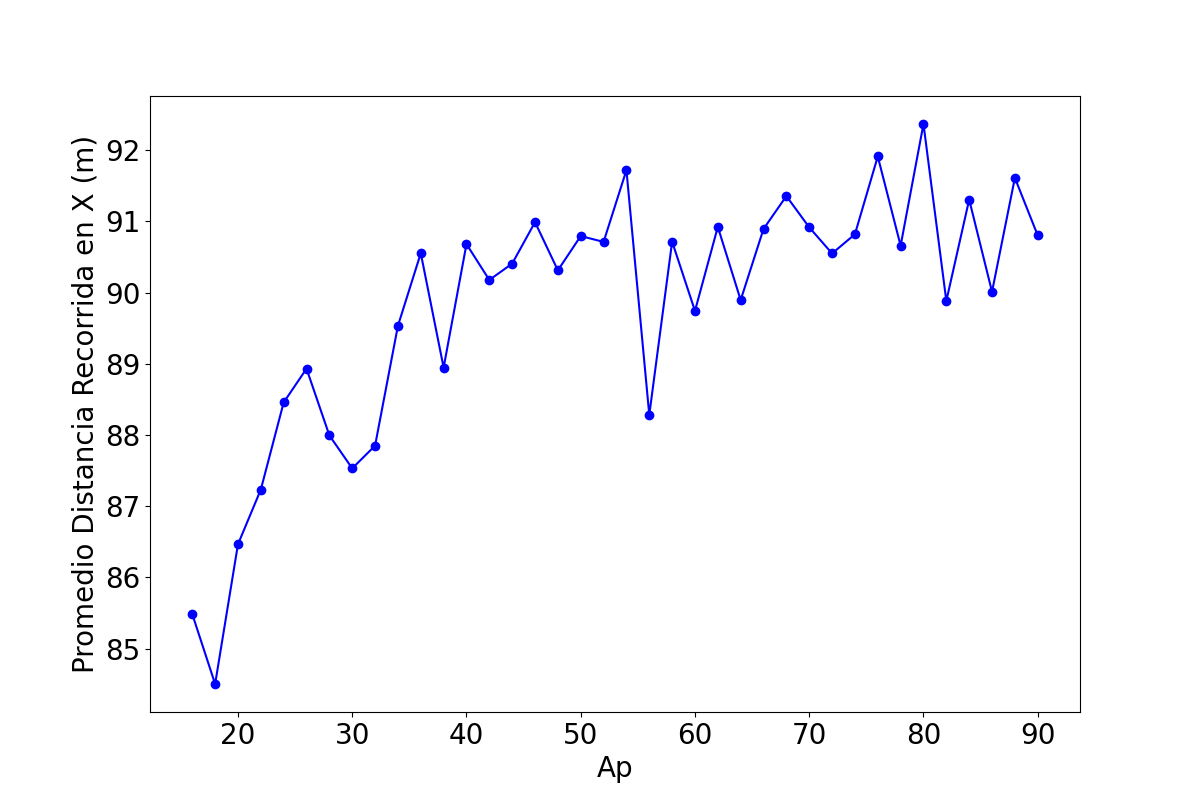
\includegraphics[width=0.75\textwidth]{pic/05-resultados/r6}
    \end{center}
\end{frame}

\begin{frame}{...}
    \begin{center}
        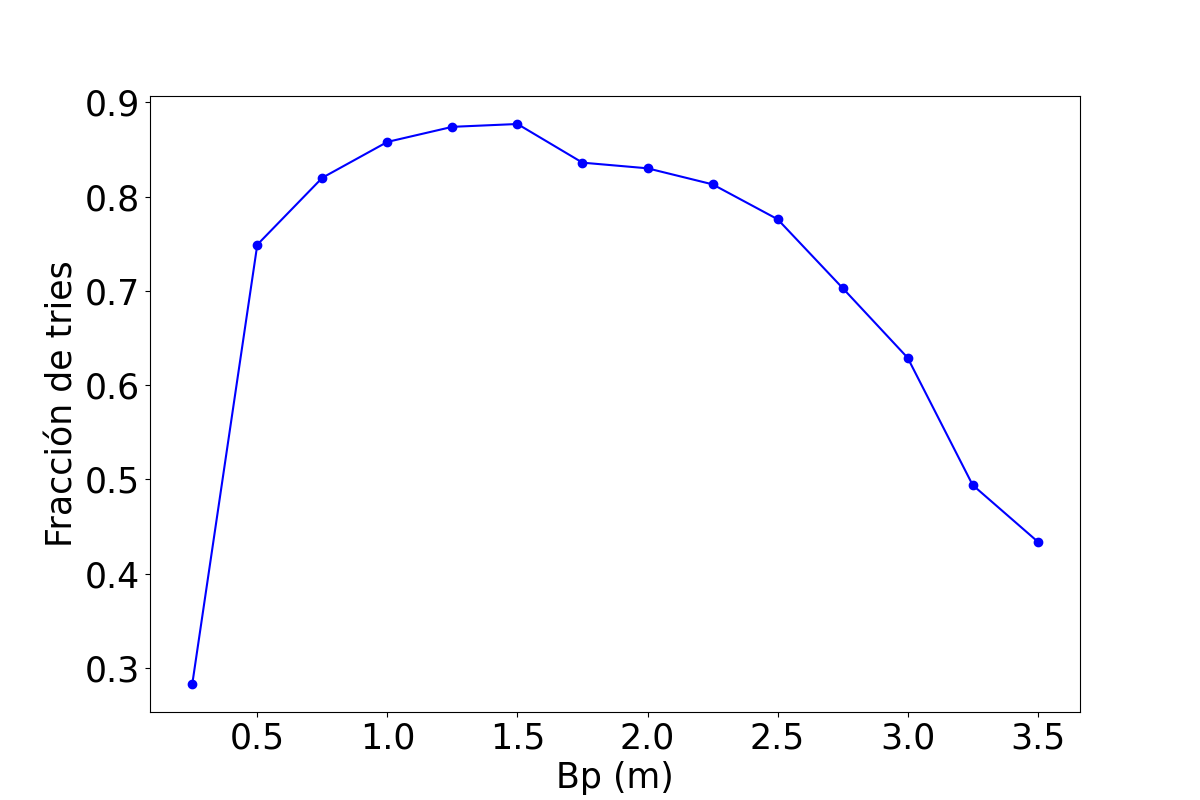
\includegraphics[width=0.75\textwidth]{pic/05-resultados/r7}
    \end{center}
\end{frame}

\begin{frame}{...}
    \begin{center}
        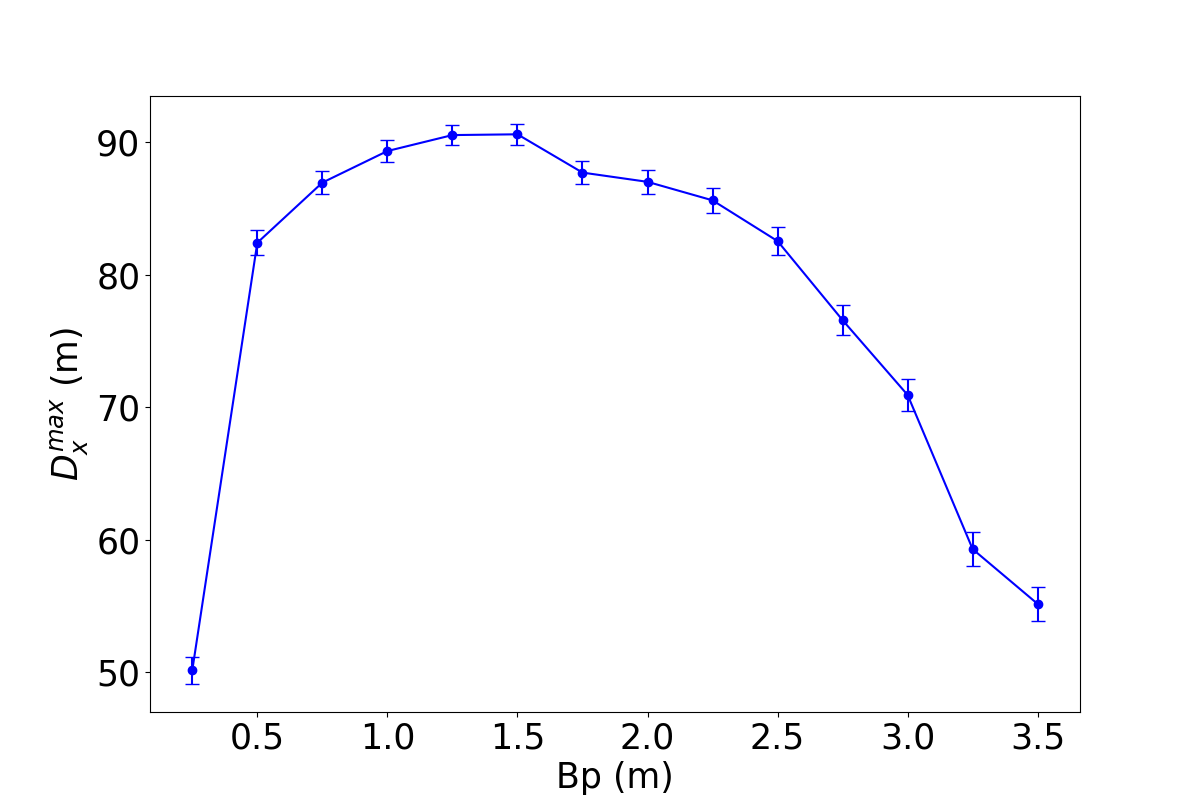
\includegraphics[width=0.75\textwidth]{pic/05-resultados/r8}
    \end{center}
\end{frame}

\begin{frame}{...}
    \begin{center}
        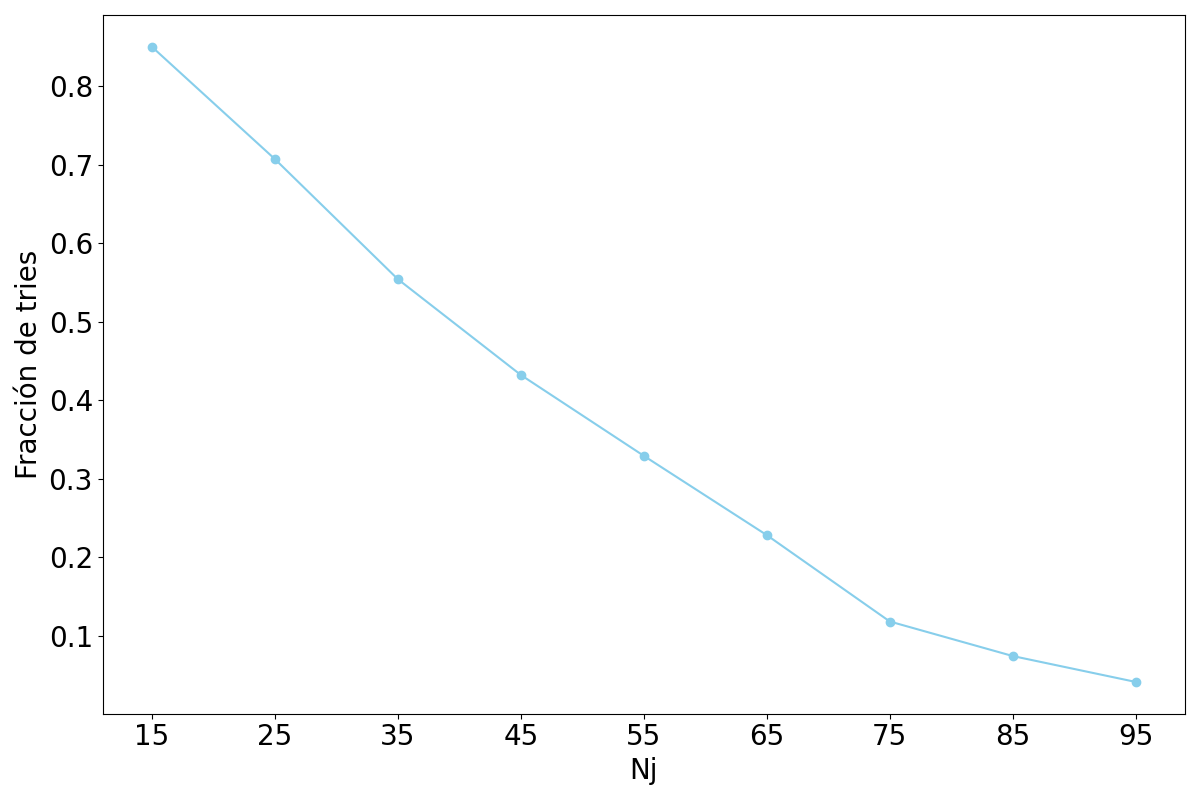
\includegraphics[width=0.75\textwidth]{pic/05-resultados/r9}
    \end{center}
\end{frame}

\begin{frame}{...}
    \begin{center}
        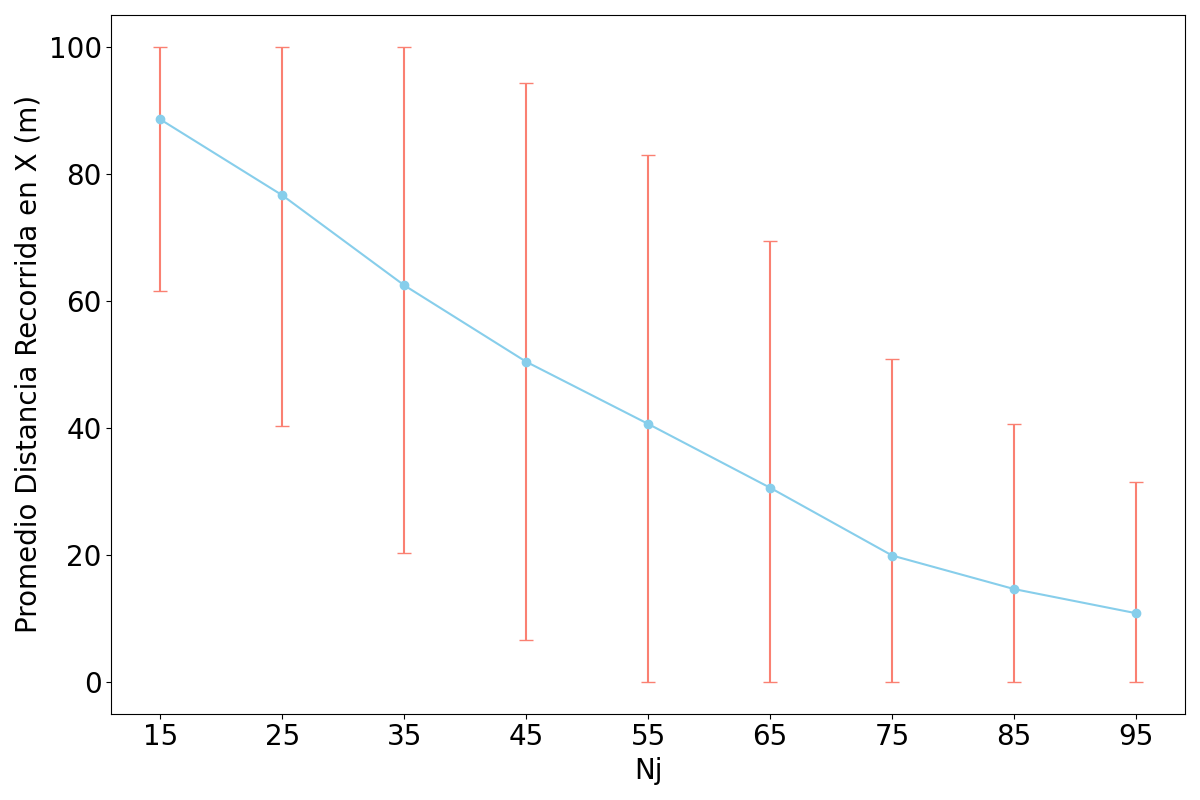
\includegraphics[width=0.75\textwidth]{pic/05-resultados/r10}
    \end{center}
\end{frame}

\begin{frame}{...}
    \begin{center}
        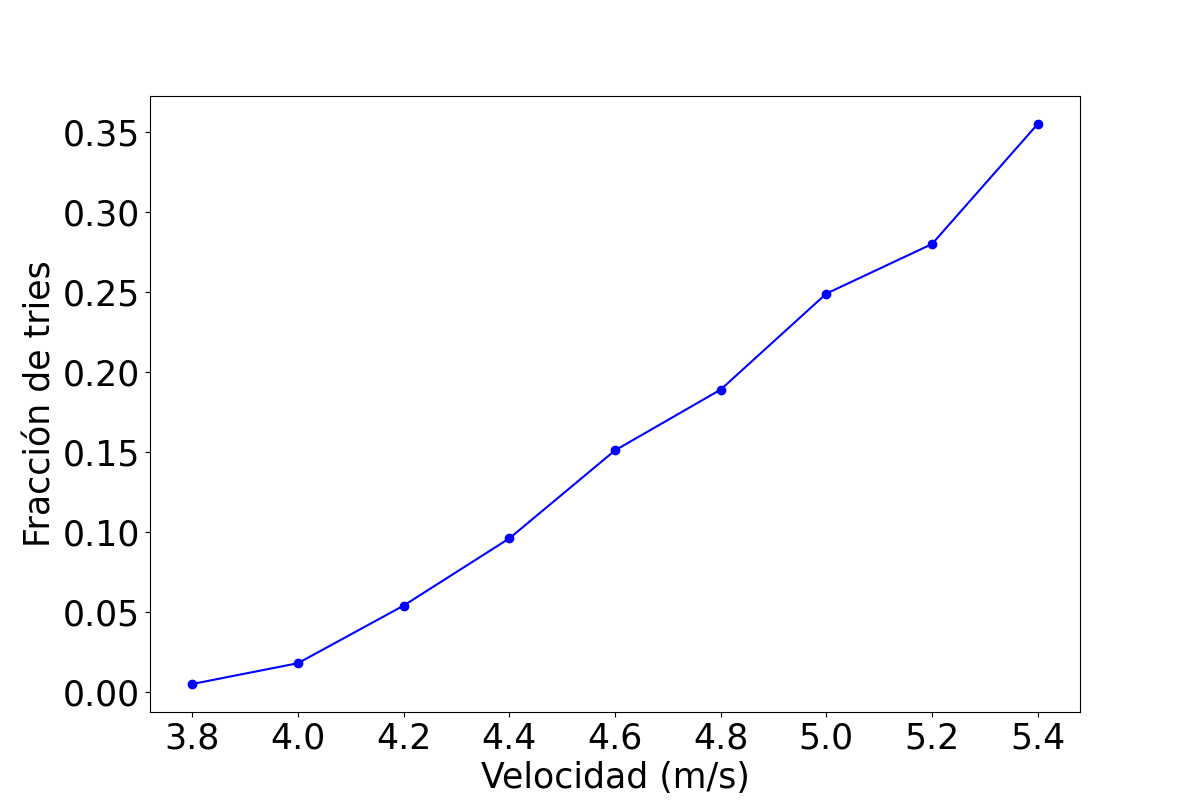
\includegraphics[width=0.75\textwidth]{pic/05-resultados/r11}
    \end{center}
\end{frame}

\begin{frame}{...}
    \begin{center}
        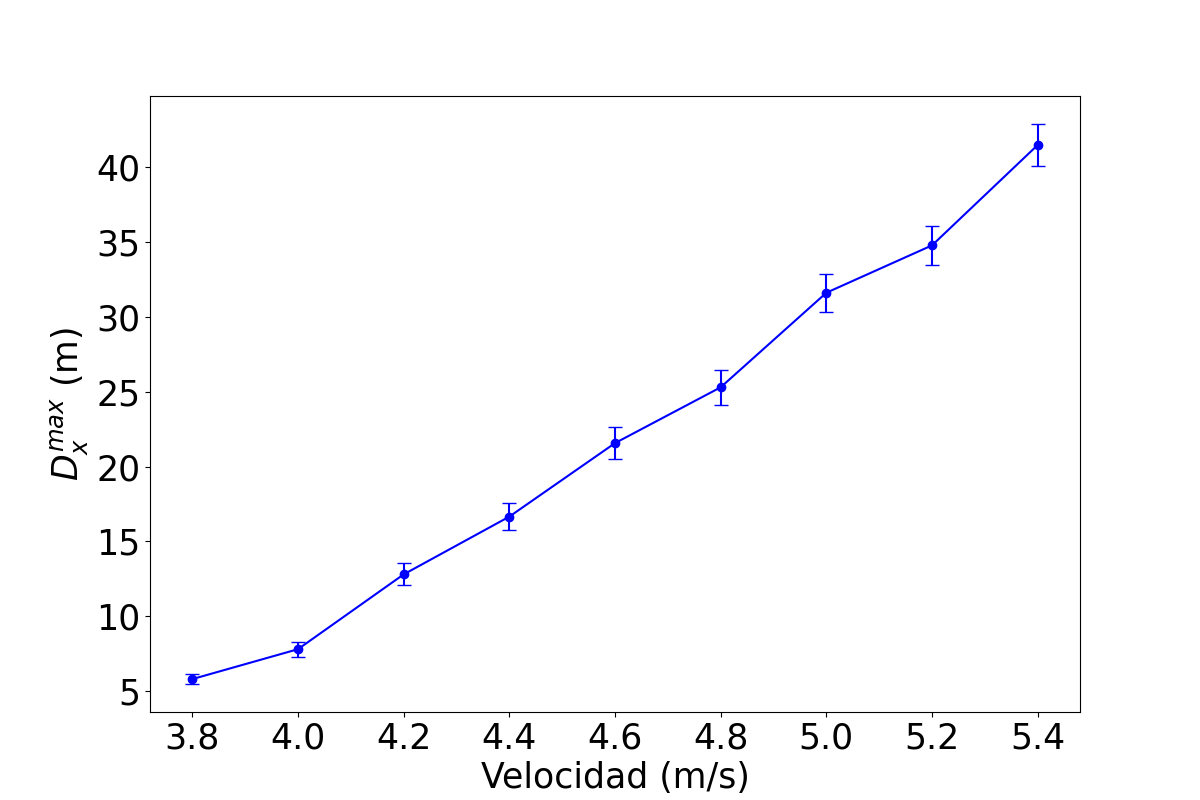
\includegraphics[width=0.75\textwidth]{pic/05-resultados/r12}
    \end{center}
\end{frame}

    \section{Conclusiones}\label{sec:conclusiones}

\subsection{Conway en 2D}\label{subsec:conway-en-2d-conc}

\subsection{Cuarentena en 2D}\label{subsec:cuarentena-2D-conc}

Si se necesitan más de 3 vecinos existe una imposiblidad de crecer más allá de su rango inicial (más o menos en realidad).

\subsection{Expansión Circular en 2D}\label{subsec:expansion-circular-2D-conc}

Something something para tener un crecimiento constante hacia todos lados no es siempre necesario que todas las celdas revivan por cualquier
cantidad de vecinos.

\subsection{Expansión Cúbica}\label{subsec:cubito-3D-conc}

Something something si es fácil que se muera con muchos vecinos quizás es mejor tener una densidad baja si se pretende crecer rápidamente.

%% Literature Review --- --- --- --- --- --- --- --- --- --- ---
\section{Modelo}
\begin{frame}{Research gap}

   this is a Literature gap.

\end{frame}

\begin{frame}{Research question}

   this is a Literature Review.

\end{frame}

% Methods --- --- --- --- --- --- --- --- --- --- ---
\section{Implementacion}
\begin{frame}{Title}
    \begin{itemize}
        \item different themes which are usable in practice
    \end{itemize}
\end{frame}

\begin{frame}
	\frametitle<presentation>{Figures}
	\begin{figure}
		\centering
			
\includegraphics[height=5cm]{pic/itba.png}
		\caption{Logo of the university.}
		\label{fig:unilogo}
	\end{figure}
\end{frame}


% Results --- --- --- --- --- --- --- --- --- --- ---
\section{Simulaciones}
\begin{frame}
    \begin{itemize}
        \item different themes
        \item different themes
        \item different themes
        \item different themes
    \end{itemize}
\end{frame}

% Results --- --- --- --- --- --- --- --- --- --- ---
\section{Resultados}
\begin{frame}
    \begin{itemize}
        \item different themes
        \item different themes
        \item different themes
        \item different themes
    \end{itemize}
\end{frame}

% Results --- --- --- --- --- --- --- --- --- --- ---
\section{Conclusiones}
\begin{frame}
    \begin{itemize}
        \item different themes
        \item different themes
        \item different themes
        \item different themes
    \end{itemize}
\end{frame}


% --- Thank you slide ---
    \begin{frame}
        \begin{center}
            \LARGE
            { ¡Muchas gracias por escuchar! }
        \end{center}
    \end{frame}

\end{document}